\chapter{Simple Network Management Protocol}\label{ch:snmp}
Large networks has too many components to be managed by human agents alone. Network devices have to maintain a large amount of management data such as configuration information,  operational state and statistics. Management information can be used to understand how a network performs, how devices in a network are configured and to change their configuration. The Simple Network Management Protocol (SNMP) \cite{rfc3410} is an application layer protocol that facilitates the exchange of management information between network devices. It exposes management data in the form of variables on the managed systems, which describe the system configuration. Since its first publication in 1988, the SNMP protocol has become the most widely-used network management tool for IP-based networks.

Currently, there are three versions of SNMP defined. The first version (SNMPv1) is nowadays a historical IETF standard, although it is still widely supported by many vendors. One of the most important weaknesses of SNMPv1 is the lack of adequate mechanisms for securing the management function. Its security is based on a community string, which is a type of password transmitted in cleartext. SNMPv2 extended the functionality of SNMPv1 and includes a number of improvements, such as additional protocol operations. A new security system was proposed, however, it was too complex and was not widely accepted. SNMPv3 addresses the security problems of the previous versions. The SNMPv3 architecture introduces a well defined extensible architecture and the User-based Security Model (USM) for message security.

The SNMP protocol is datagram-oriented and its implementation can be very lightweight \cite{draft-6lowpan-snmp}. It can fit resource-constrained devices very well. This makes it a perfect candidate as a management protocol for 6LoWPAN applications. In this chapter an overview of the SNMPv3 protocol is given.

\section{Protocol Architecture}
The SNMP protocol is designed to have a modular architecture, which allows the evolution of the protocol and enables protocol extensions. The protocol architecture is composed of an SNMP engine and applications. An SNMP entity is an implementation of this architecture. The SNMP engine includes several subsystems communicating via defined abstract service interfaces. Abstract service interfaces describe the conceptual interfaces between various subsystems.  While the subsystems can be changed and extended over time, the interfaces are fixed.

\begin{figure}[htp]	
\begin{center}
    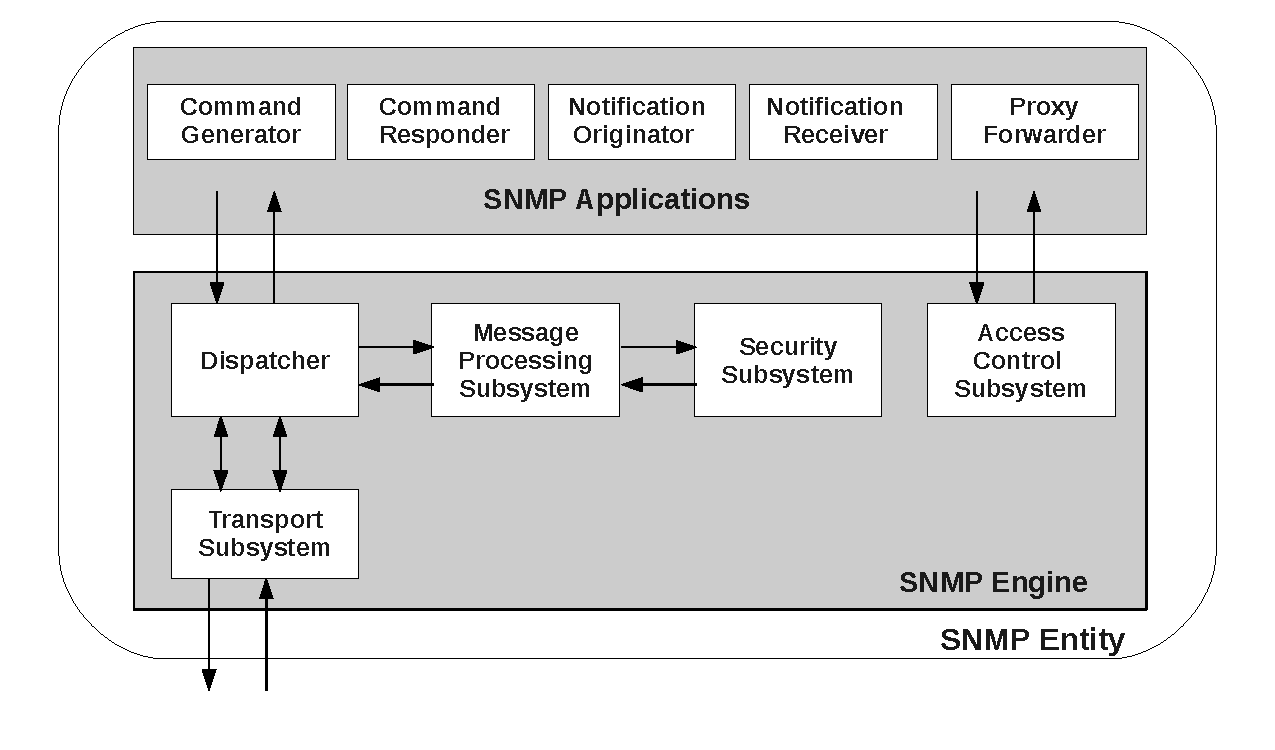
\includegraphics[scale = 0.6]{img/snmp-arch.pdf}
    \caption{Structure of an SNMP entity}   
	\label{fig:snmparch}
\end{center}
\end{figure}

According to the SNMP architecture defined in \cite{rfc3411}, the SNMP engine is composed of a dispatcher, a message processing subsystem, a security subsystem, an access control subsystem, and a transport subsystem (Figure \ref{fig:snmparch}). Each subsystem may include multiple concrete models implementing different services. The dispatcher is the key part of an SNMP engine. It's responsible for controlling the data flow within an SNMP entity. When an SNMP message needs to be prepared or when data needs to be extracted from an SNMP message, the dispatcher delegates these tasks to a version-specific message processing model within the message processing subsystem. It also dispatches SNMP  protocol data units (PDUs) to SNMP applications. Each message processing model defines the format of a particular version of an SNMP message. Typically, the message processing subsystem supports three models for SNMPv1, SNMPv2c, and SNMPv3. The security subsystem provides security services such as authentication and privacy of messages. Authorization services are provided by the access control subsystem. The transport subsystem \cite{rfc5590} allows for multiple transport protocols to be used.

There are several types of defined applications (Figure \ref{fig:snmparch}), such as a command generator which monitor and manipulate management data, a command responder providing access to management data, a notification originator initiating asynchronous messages, a notification receiver processing these messages, and a proxy forwarder which forwards messages between entities. Applications may use the services provided by the SNMP engine. An SNMP entity which includes one or more command generator and notification receiver applications is called an SNMP manager. An entity containing one or more command generator and notification receiver applications is called an SNMP manager.

\section{Message Format}\label{sec:messformat}
The SNMPv3 message (Figure \ref{fig:snmp-format}) contains the SNMP version, fields for global data (such as the message identifier, the maximum message size, the security model and the level of security), fields for the security model information and naming scope (context identifier and name), and finally the protocol data unit (PDU).
\begin{figure}[htp]	
\begin{center}
    \includegraphics[scale = 0.60]{img/snmpv3-message.pdf}
    \caption{SNMPv3 message format}   
	\label{fig:snmp-format}
\end{center}
\end{figure}

The SNMP Version field identifies the version of the message processing. The message identifier (msgID) is used between two SNMP entities to coordinate request messages and responses and to coordinate the message processing by different subsystem models. The maximum message size (Max Size) is the maximum message size supported by the sender of the message, i.e., the maximum message size that the sender can accept when another SNMP engine sends an SNMP message. The Flag field contains several bit fields which control processing of the message. The security model field enables the concurrent support of multiple security models identifying which security model was used by the sender to generate the message. The security parameters field is used for communication between the security model modules in the sending and receiving SNMP engines. The contents and format of the data in this field are defined by the security model.

The naming scope contains a PDU and the context in which it has to be processed. The context engineID identifies the engine which realizes the managed objects referenced within the PDU, and the context name defines the particular context associated with the management information contained in the PDU of the message. These fields are followed by the PDU data.

\section{Protocol Operations}
As described in Section \ref{sec:messformat}, an SNMP message encapsulates a PDU which specifies the operations performed by the receiving SNMP engine. The SNMP protocol defines PDUs for the following operations: Get, GetNext, GetBulk, Response, Set, Trap, Inform.

In addition, the Report protocol operation can be used internally to allow SNMP engines to communicate with each other for error notifications and clock synchronization.



\section{Security Models}

